\section{Вероятностное пространство}

Для работы с информационными эвристиками нам нужно построить вероятностное пространство для каждого слоя. Пространства входа $X$ и выхода $Y$ не изменяются в зависимости от эпохи обучения. При этом латентное пространство $Z$ будет менятся с каждыми новыми весами моделей. \\
\subsection{Вероятностное пространство на выходном слое}
Проше всего задать вероятностное пространство на выходном слое, так как это категоричный признак, он принимает только целые числа в отрезке [0, 9]. Cоотвенственно если данные в семплах распредены равномерно, то вероятность выпадания каждого класса - 0.1. проверим это посчитав количествено все метри на датасете.
\begin{center}
    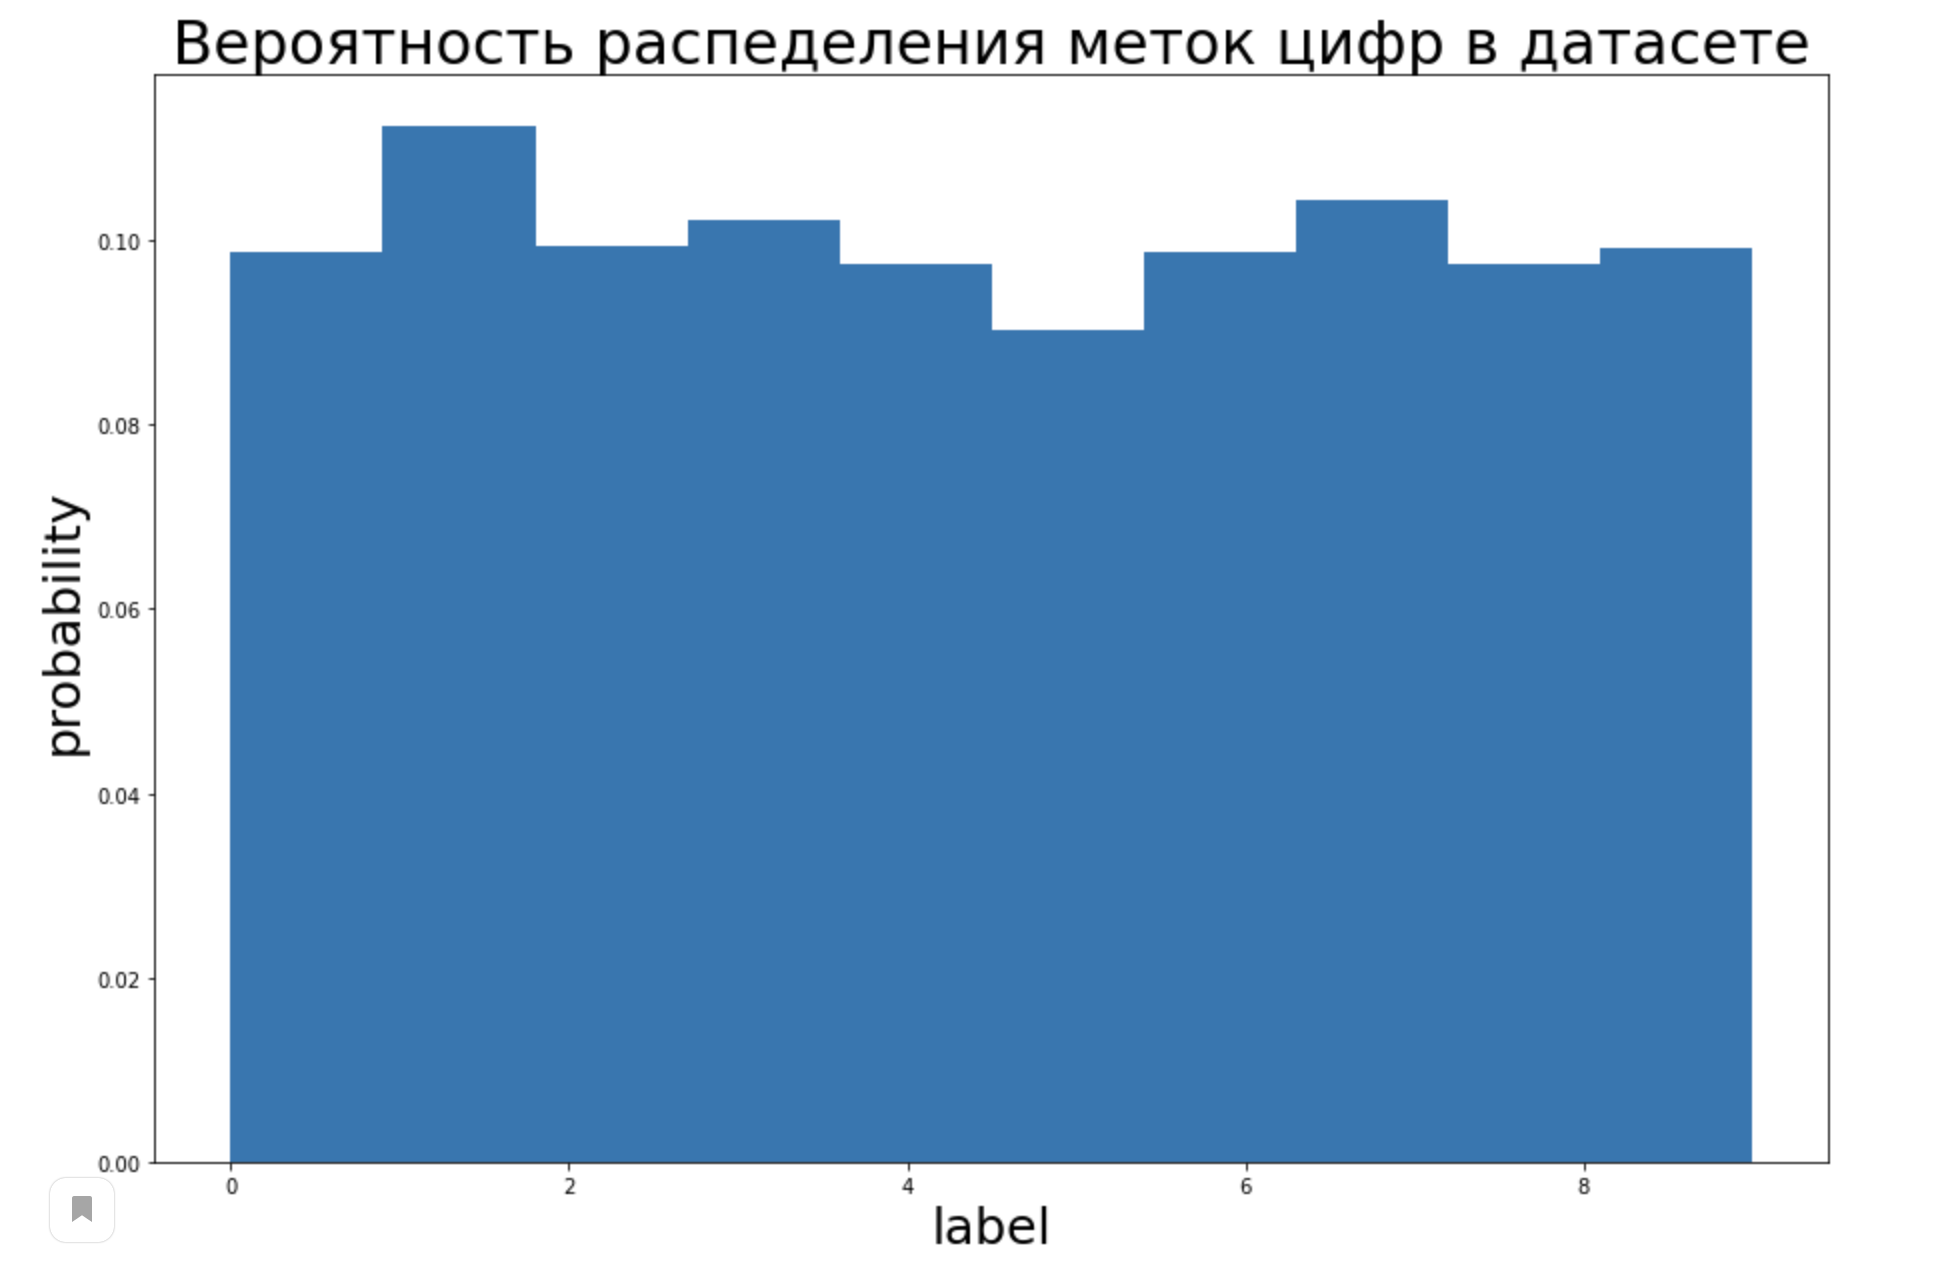
\includegraphics[scale=0.4]{images/y_prob.png}
\end{center}
Как видно на графике распределение на выходном слое почти равномерное, будем считать что вероятность для каждого элемента будет 1 / 10.
Сложнее ситуация с пространства входа и латентными, так как они многомерные.
\subsection{Вероятностное пространство на входном слое}
Сначала разберемся с входным пространством. Его размерность $(samples\_count, 1, 28, 28)$. Рассмотрим конкретную координату картинки и посмотрим как распределены значения на конкретном признаке. \\
В качестве примера возьмем координаты (14, 14) и (7, 7):
\begin{center}
    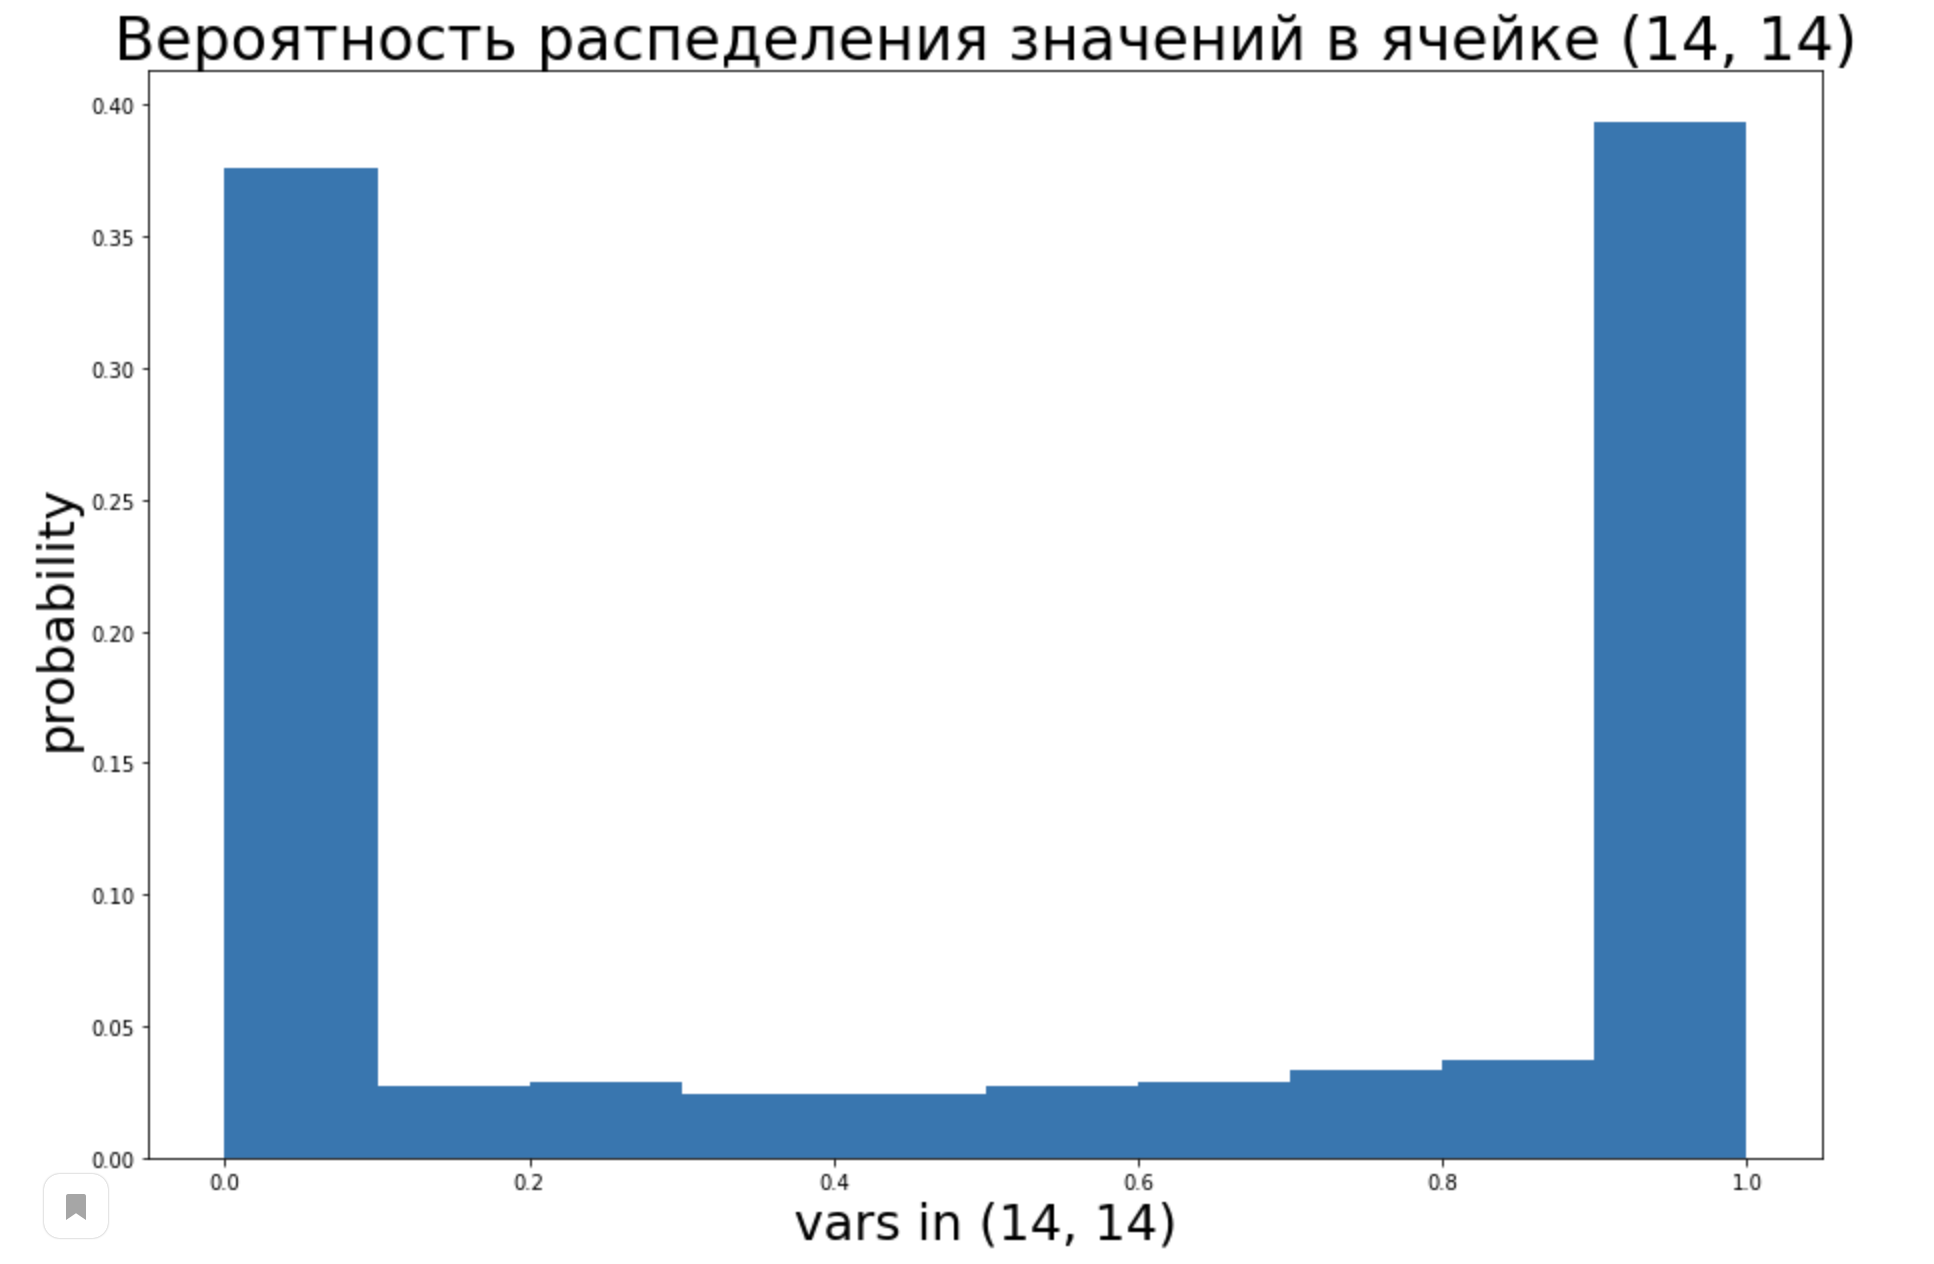
\includegraphics[scale=0.4]{images/x_(14, 14).png}
\end{center}
\begin{center}
    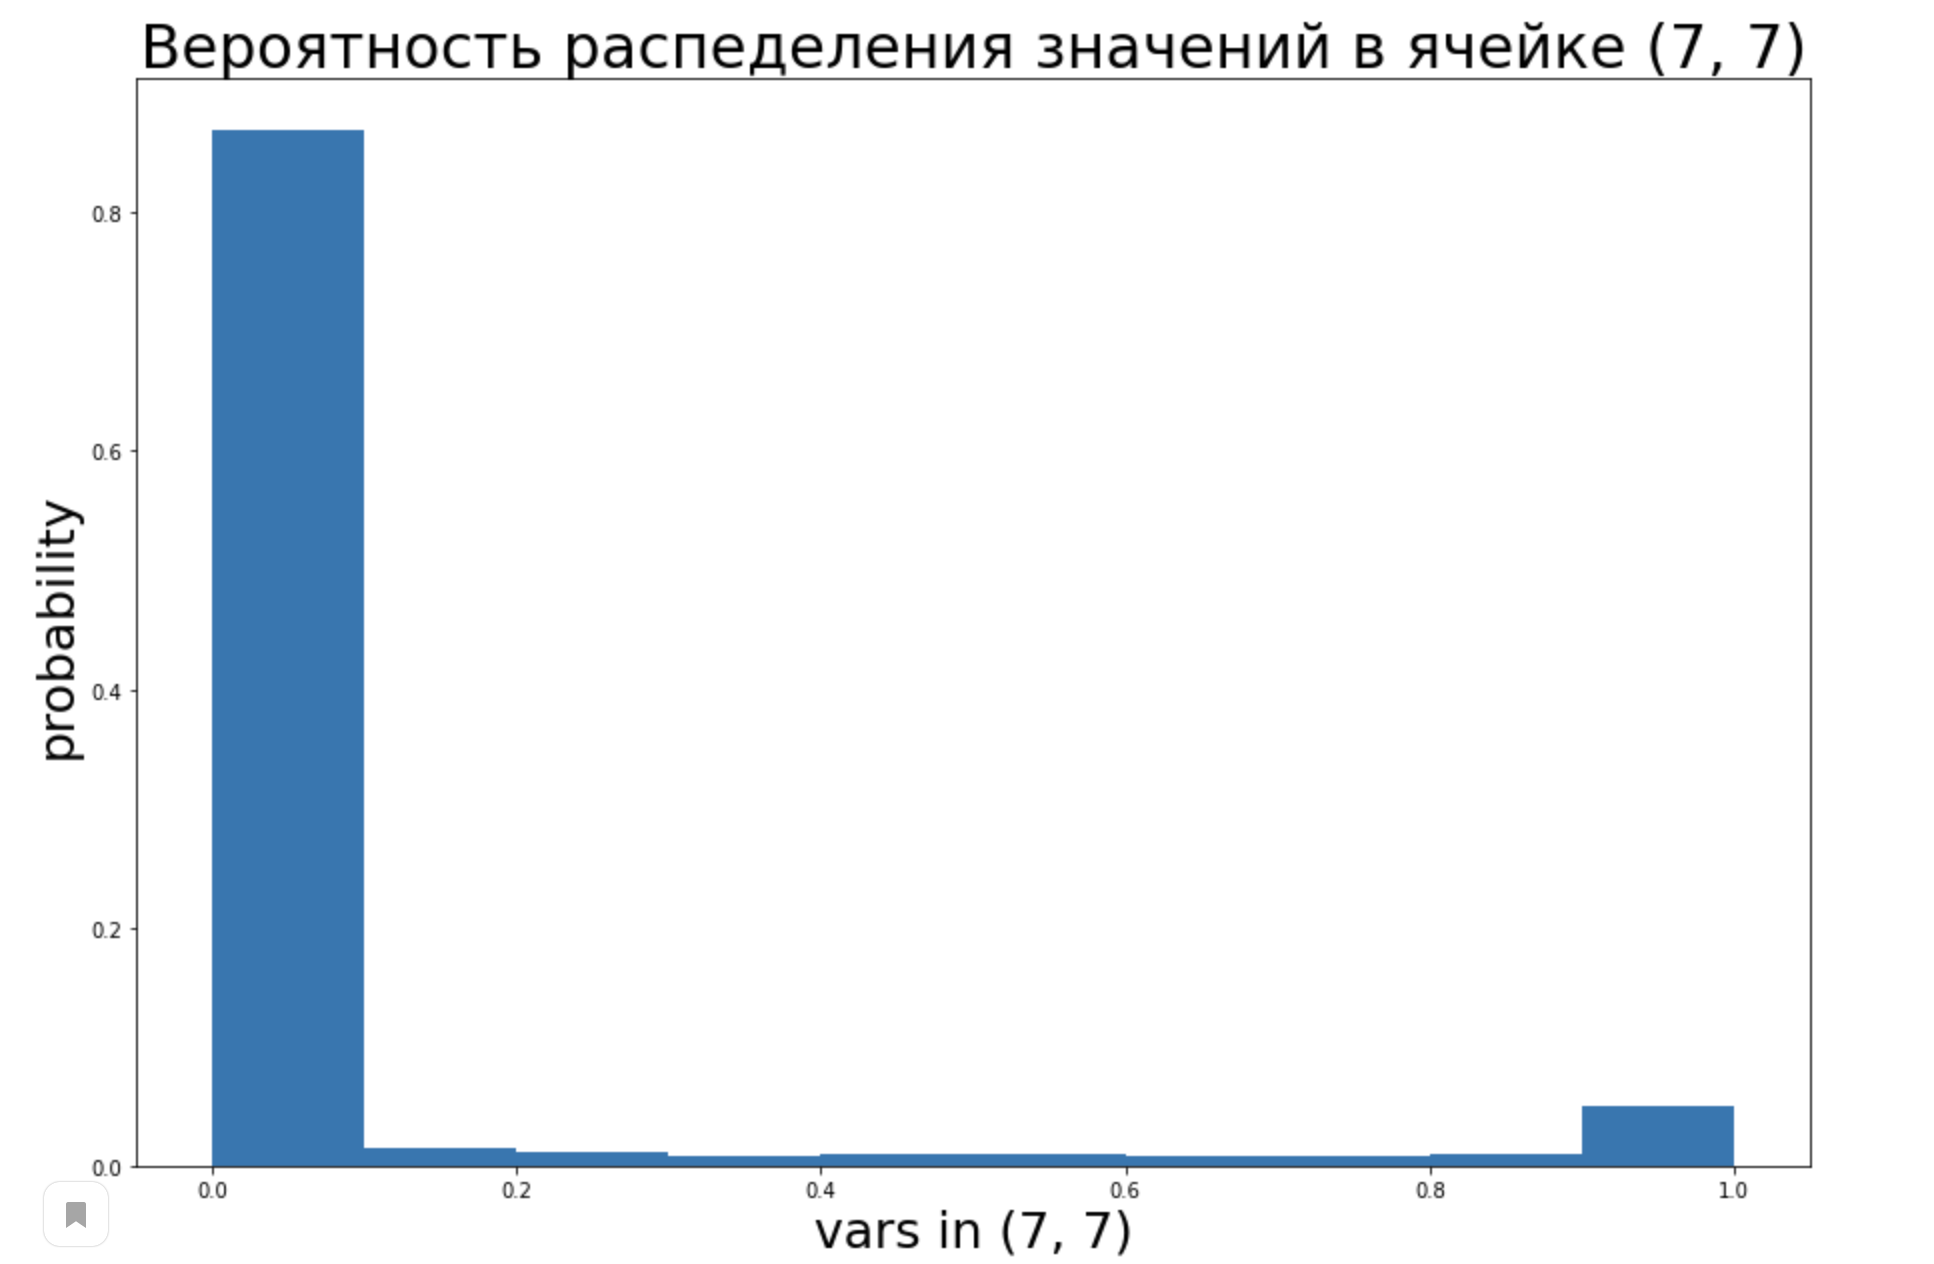
\includegraphics[scale=0.4]{images/x_(7, 7).png}
\end{center}
Видно, что значения внутри каждой ячейки распределены нестандартно, привалирующие значения - 0 и 1. Также правильнее рассматривать модель, где значения в каждой ячейке зависят друг от друга, так как картинки являются не случайным шумом, а непрерывными матрицами, то есть если все значения вокруг ячейки равно 1., то скорее всего значение в ячейки тоже 1. Проверим этот факт независимости. \\
Возьмем квадратик из 4 ячеек и проверим вероятность условия, что все значения больше 0.5 и также посчитаем перемноженную вероятность что значение в каждой ячейке больше 0.5 и сравним эти значения
\begin{gather}
\begin{aligned}  
P(x_{i,j} > 0,5, x_{i,j+1} > 0,5, x_{i+1,j} > 0,5, x_{i+,j+1} > 0,5) \\
? \\
P(x_{i,j} > 0,5), * P(x_{i,j+1} > 0,5) * P(x_{i+1,j} > 0,5) * P(x_{i+,j+1} > 0,5)
\end{aligned}
\end{gather}
Рассмотрим конкретный пример, описанный выше со значениями i = 14, j = 14
\begin{center}
    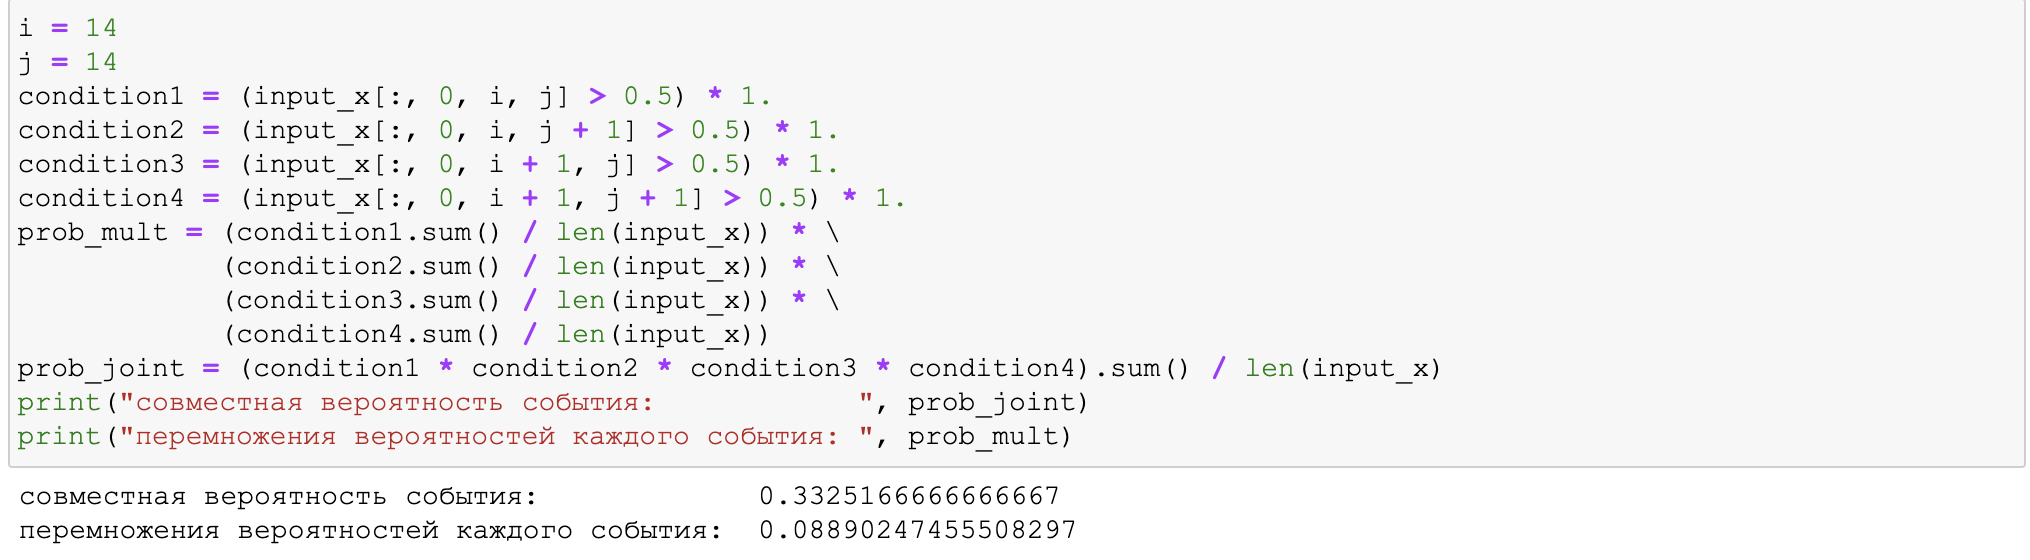
\includegraphics[scale=0.6]{images/x_independency.png}
\end{center}
Как видно на примере значения совершенно различные что говорит о зависимости между признаками входа. \\
Для удобства дискретизируем все значения входа, так как значения на входе принимают вещественные значения на отрезке [0, 1]. Четкое количество кусков разбиения оставим в качестве гиперпараметра и подберем при валидации. При дикретизации мы будем иметь дело с конечным пространством, что удобнее. Пример такой дискретизации:
\begin{gather}
\begin{aligned}  
X_{discrete} = (X_{input} > 0.5) * 1.
\end{aligned}
\end{gather}
Данная дискретизация приводит все значения к двум полярным - 0 и 1, данная дикретизация нам подходит, так как на примерах распределения значений по признакам значения с наибольшими вероятностями были именно полярные значения. \\
На данный момент непонятно какими вероятнострыми моделями приближать такие сложные многомерные пространства как входное, поэтому наилучшим решением будет рассматривать исходы как элементы построенного дискретного пространства. Может быть проблема, что каждый элемент датасета будет инъективно отображаться в построенное дискретное пространства, для проверки этого посчитаем количество различных исходов. Пусть количество параметров при дискретизации будет минимально, а именно 2. То есть все входные значения переходят либо в 0 либо в 1. В таком случае полученное пространство будет иметь $2^{28*28}$ различных исходов, тем временем количество элементов в датасете 60000, что на много порядков меньше чем $2^{28*28}$. Для решение этой проблемы используем искуственное сжатие пространства, которое рассмотрим чуть позже.
\subsection{Вероятностное пространство на латентных пространствах}
Для начала посмотрим как устроены данные на промежуточных слоях. Это также многомерные пространства, посмотрим на пример распределения одного из признаков слоя после первой свертки:
\begin{center}
    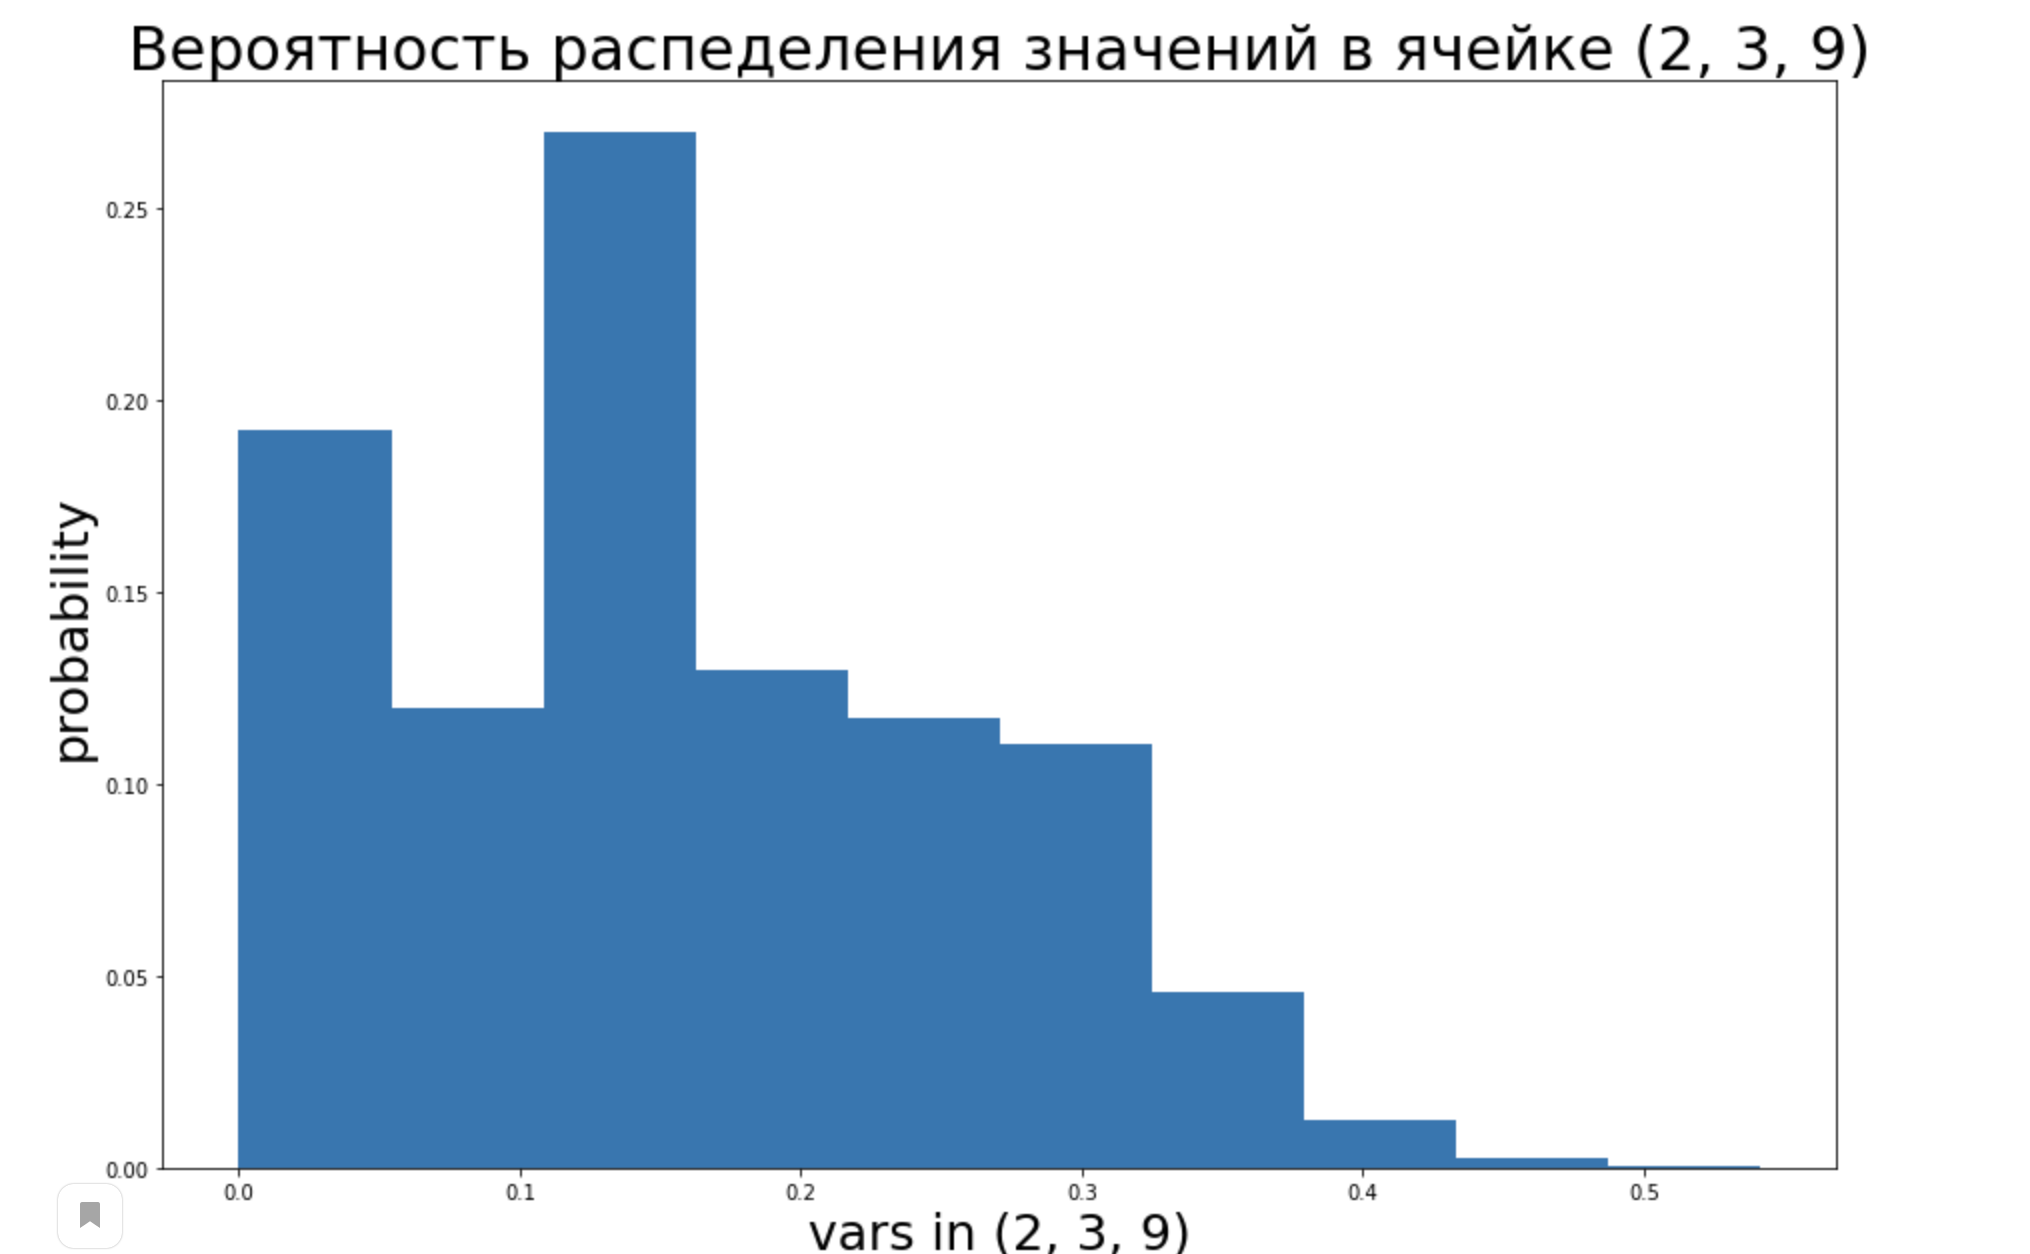
\includegraphics[scale=0.4]{images/Z1_dist.png}
\end{center}
Данные здесь получаются после применения 2d свертки, ативации RELU и после пуллинга, соответственно все данные меньшие 0 стали равны 0, можно сделать вывод что после сверки данные имели нормальное распределение с шумом, но после функции активации стали иметь распределение как у функции RELU(norm), описать стандартной моделью подобные данные не получится. \\
Также данные будут зависимы друг с другом по призакам, так как значения в латентных слоях являются функцией от входных данных, которые выполняются на forward pass. Так как forward pass будет работать почти инвариантно на первых слоях сети из-за больших размеров пространств зависимость созраняется. \\
Соответственно для построения латентного пространства мы также проводим дискретизацию, чтобы привести непрерывное пространство в конечное. Для этого мы находим квантили распределения (например 0.01 и 0.99 квантиль) и ограничиваем нашу область по признаку этой квантилью. Значения будут находится за ее пределами с вероятностью $0.01 + (1 - 0.99) = 0.02$. Далее разбиваем полученный отрезок на несколько равномерных кусков и дискретизируем. Количество кусков оставим в качестве гиперпараметра и подберем его при валидации. \\
При расчете полученного пространства после дискретизации возникают те же проблемы, что и на входном пространстве. Если рассматривать в качестве исходов - элементы дискретизации, то распределение получится также равномерным в силу того, что количество семплов в датасете намного меньше чем возможных вариантов исходов, поэтому прибегнем к такому же сужению пространства, поговорим про него поподробней.
\subsection{Сужение вероятностных пространств}
Как выяснилось в предъидущих пунктах, работать с вероятностным пространством без сужения будет бессмысленно, покажем это на практике в главе ниже. \\
Для снижения пространства будем использовать пуллинги, то есть объединение соседних признаков тензора в один. Эта операция сохраняет вероятно-признаковое пространство, так как в архитектурах сети часто используются пуллинги (как например в нашей сети классификации цифр по картинке). Особенности пуллинга также будем использовать как гиперпараметр. \\
Для двумерного пространсва такого как нащи исходные данные будем использовать $2d average pooling$. Если использовать окно 7x7 то после 
пуллинга размер матрицы будет $(28 / 7) * (28 / 7) = 16$. В таком случае количество исходов полученного вероятностного пространства будет $2^{16} = 65538$, что уже сопоставляется с размерностью исходного датасета. Уже в этом случае 
\begin{gather}
\begin{aligned}  
p(f(x_i) = f(x_j) \cap i \neq j) \ll 1, \\
f = discrete \circ pooling 
\end{aligned}
\end{gather}
Пример 2d пуллинга:
\begin{center}
    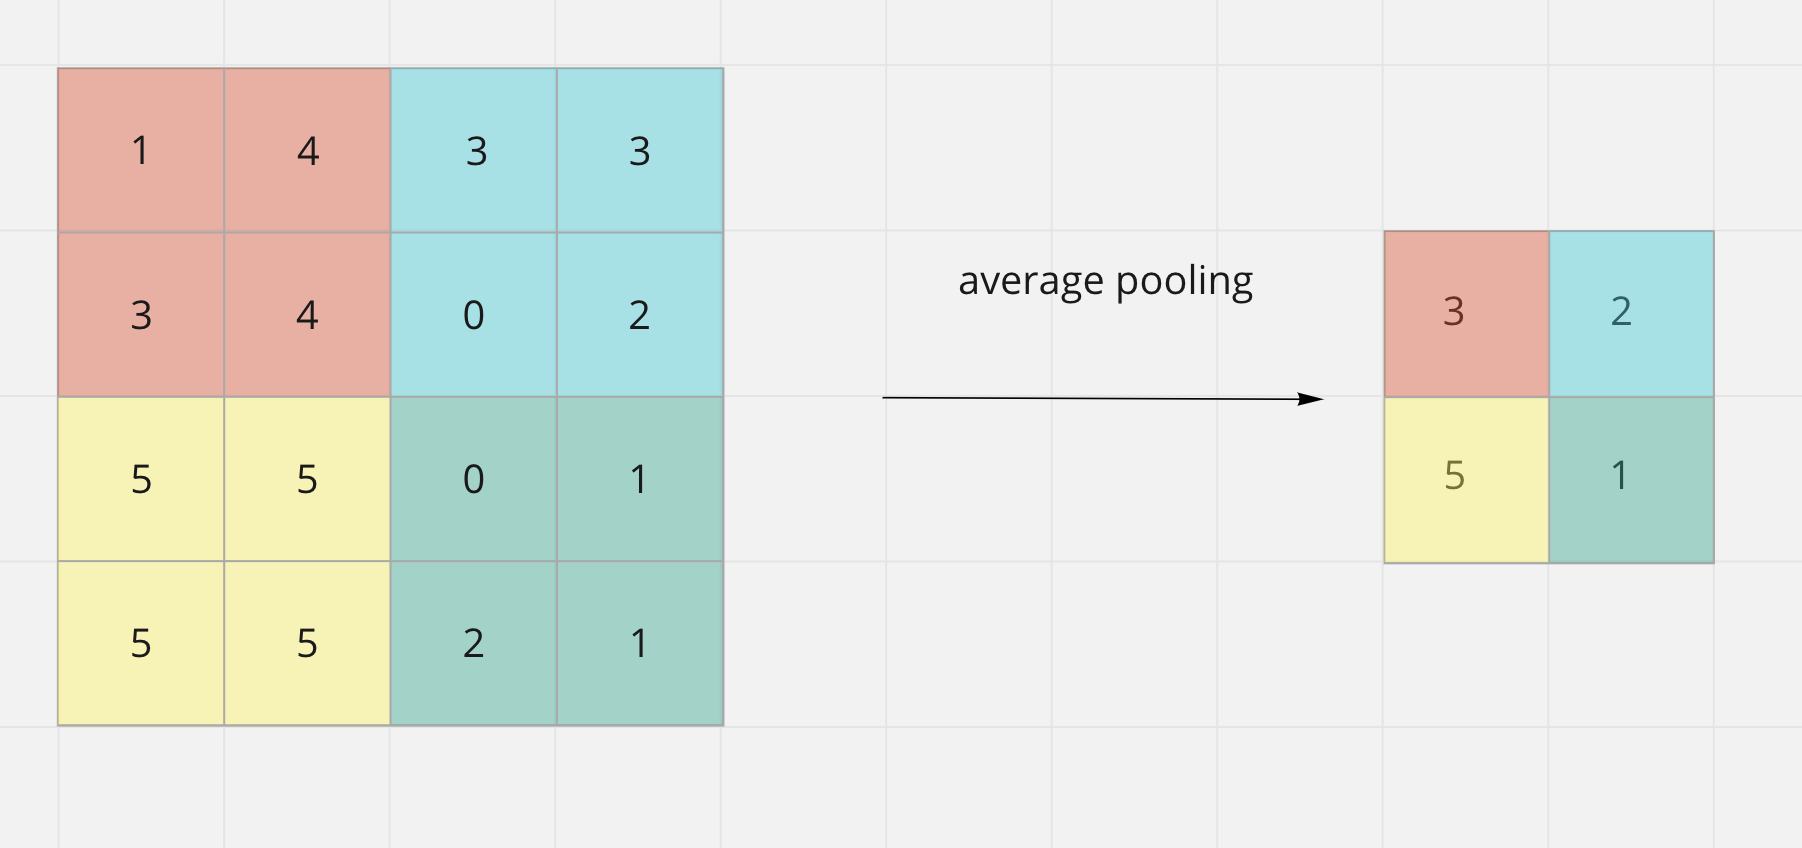
\includegraphics[scale=0.3]{images/2d_pooling.png}
\end{center}
В случае пуллинга латентных пространств мы будем использовать 3d пуллинги вместа 2d пуллингов, если новая размерность нам будет не подходить из-за все еще большого количества исходов. Соответственно в случае 3d пуллинга могут возникнуть проблемы, что пуллинг будет проходить межлу различными каналами, кторые могут быть не связаны между собой. В таком случае мы будем использовать 2d пуллинги с большим окном. \\
Пример 3d пуллинга:
\begin{center}
    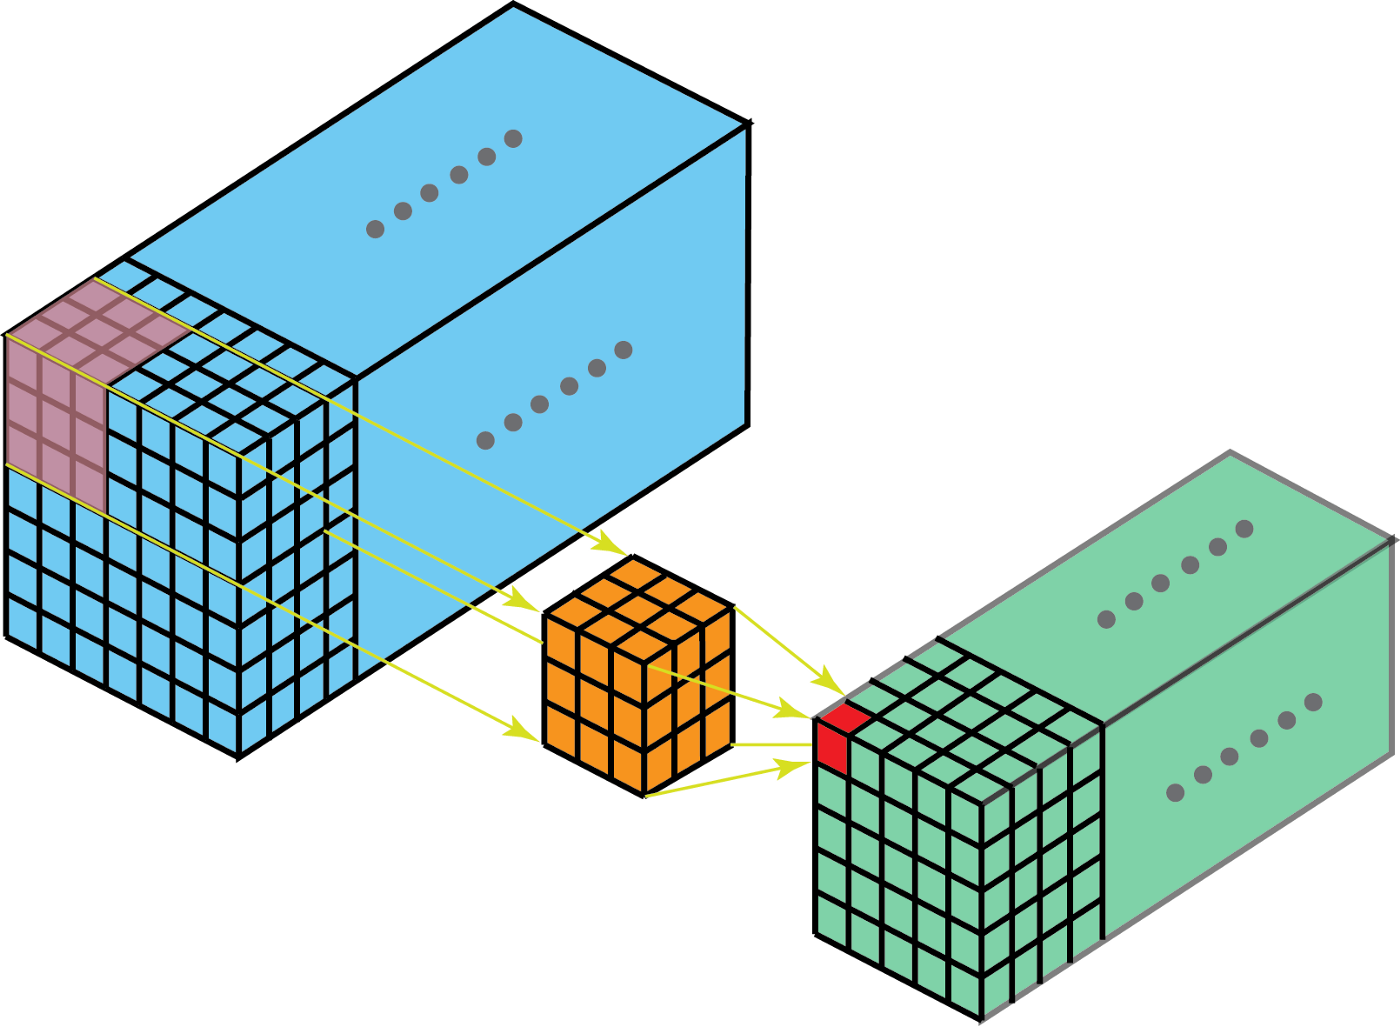
\includegraphics[scale=0.3]{images/3d_pooling.png}
\end{center}
% https://towardsdatascience.com/types-of-convolution-kernels-simplified-f040cb307c37
 